% This is samplepaper.tex, a sample chapter demonstrating the
% LLNCS macro package for Springer Computer Science proceedings;
% Version 2.21 of 2022/01/12
%
\documentclass[runningheads]{llncs}
%
\usepackage[T1]{fontenc}
% T1 fonts will be used to generate the final print and online PDFs,
% so please use T1 fonts in your manuscript whenever possible.
% Other font encondings may result in incorrect characters.
%
\usepackage{graphicx}
% Used for displaying a sample figure. If possible, figure files should
% be included in EPS format.
%
% If you use the hyperref package, please uncomment the following two lines
% to display URLs in blue roman font according to Springer's eBook style:
%\usepackage{color}
%\renewcommand\UrlFont{\color{blue}\rmfamily}
%
% \usepackage{wrapfig}
%
\begin{document}
%
\graphicspath{ {./figs/} }
%
\title{Orchestrating information governance workloads as stateful services on clouds using Kubernetes Operator Framework}
%
%\titlerunning{Abbreviated paper title}
% If the paper title is too long for the running head, you can set
% an abbreviated paper title here
%
\author{First Author\inst{1}\orcidID{ 0000-0002-2816-2699}}
%
\authorrunning{C.Mega}
% First names are abbreviated in the running head.
% If there are more than two authors, 'et al.' is used.
%
\institute{University on Stuttgart, Stuttgart, Germany
\email{cataldo.mega@ipvs.uni-stuttgart.de}\\
\url{https://www.ipvs.uni-stuttgart.de/departments/as/}}
%
\titlerunning {IG Workloads on Clouds} 
\maketitle              % typeset the header of the contribution
%
\begin{abstract}
The proliferation of unstructured data, and information stored within an enterprise is a challenge for organizations due to increasing regulation and compliance. Creating, capturing, managing, storing and accessing information requires substantial IT investment. Information volume doubles ever 2 years and e-Discovery consumes as much as ½ of the litigation budget in an Enterprise given that data storage cost increases faster than disposal takes place. Due to regulations the average cost paid for lost or stolen sensitive records and confidential information is steadily increasing. This means without a holistic Enterprise Information Management (EIM) strategy that includes Information Governance (IG), data has little value whereas cost and risk increases. The conclusion is to enhance Enterprise Information Management (EIM) with IG. Exploiting Information Lifecycle Governance (ILG) improves the information economics for organizations and complements Enterprise Information Management.

\keywords{Enterprise Information Management \and Information Governance \and Cloud-Services}
\end{abstract}
%
\section{Introduction}

Enterprise Information Management (EIM) aims at managing all data and information across an enterprise driven by 3 fundamental business metrics value, cost and risk. The Data lifecycle begins with the creation and extends through till disposition of data. 
Records are the companion of data, they represent governance metadata created through the Records Lifecycle Management (RLM) and its components. Records refer to the creation, classification, maintenance, and disposition of data and information. Records metadata assign an appropriate information governance context and adequate storage policies to data.

Information Governance (IG) and consists of implementing an Information Governance Program (IGP) that allows to steer information lifecycles based on actual data value, cost and risk. As such, Information Lifecycle Governance (ILG), through workflows uses analytics to determine and maximize value as context erodes. ILG processes enforce archiving of data onto hierarchical storage to ensure storage cost declines as value declines and trigger disposal to avoid cost and eliminate risk when data is no longer needed.

\subsubsection{Usage Scenarios}
Before presenting IG workloads lets discuss briefly what IG is all about. 

In summary the business requirements of Information Governance consist of business and regulatory compliance needs based on standards and the controls related to information lifecycle, access, retention and disposition aiming at minimizing risk through the use of up-to-date technology and efficient operations. From what was said so far we can define the following 5 use case scenarios and implied workloads:

\begin{enumerate}
    \item Collect and pre-classify enterprise data 
    \item Store, index and secure data in the enterprise repository.
    \item Search and Access data.
    \item Records Management: classification, retention, hold and dispose of data
    \item e-Discover and serve legal requests aggregating and transferring data on hold
\end{enumerate}

....

\subsubsection{IG Solutions Blueprint}



 \section{Problem Description}

Traditional ECM solutions are developed as monolithic applications and must be decomposed for running on cloud platforms. They are typically deployed on bare metal or at most in virtualized IT infrastructures. They do lack to support for CI/CD and can not be cost-effectively operated in scale-out environments. Key Cloud benefits are exploitation of elastic infrastructures to better cope with fluctuating workloads. There is no upfront capital expenditure (CAPEX) and allow a 
high degree of automation (Software Defined Infrastructure - SDI) which translates in reduced operational costs (pay-per-use pricing models). Thus the fundamental problem is how to efficiently migrate legacy ECM solutions components and its stateful services on to cloud environments.

\subsection{ Solutions Approach}

Design how to orchestrate stateful IG governance workloads using Kubernetes Operator Pattern Implement, deploy and test a prototype of stateful DB2 database services Design a Kubernetes cluster of DB instances running in Docker containers providing:
High Availability and Disaster Recovery
Develop a Kubernetes operator for DB2 using Kubernetes Operator SDK
Deploy and manage the cluster lifecycle by Kubernetes automatically

\subsection{ Decomposing a monolithic IG Solution  }

\begin{enumerate}
    \item Decompose monolithic Solution
    \item Create independent components and classify into 'Stateless' and 'Stateful'-Groups 
    \item Create a deployment topology 
\end{enumerate}

\section{Foundation}

\subsection{Workload Management Concepts}
A workload can be seen as a representative mix of primitive operation performed against a system. As an example, if we observe the typical behavior of a number of interactive compliance archive users we would see that these end users perform a number of tasks in a given time frame. For example: The end user would log on to the archive, then navigate to its workplace and open his in-workbasket. Next he picks a work item, let say an insurance claim and would start reading the claim. A few minutes later, he opens the Search UI and performs a search against the archive to find collateral documents relevant to the claim. The search yields a hit list with 20 documents, out of which he selects to retrieve 3 one after the other and annotates the 3rd updating the document. After many iterations of the same mix of operation he eventually log out of the system       

Using our example above we can synthesize the workload into a mix of primitive operations described as:

\begin{enumerate}
    \item a representative mix of Create, Retrieve, Update, Delete operations 
    \item a number of simple and complex search operations
    \item a typical corpus of data consisting of document of certain types and sizes
\end{enumerate}

\begin{table} [ht]
 \centering
    \begin{tabular}{c|c|c|c|c|}
    \hline
         Workload Element &  Primitive Operation & Payload & KPI & SLA \\ \hline
         Interactive & Create    & 100KB & Resp.Time  & 1 s   \\
                     & Retrieve  & 100KB & Resp.Time  & 1 s   \\
                     & Update    & 100KB & Resp.Time  & 1 s   \\
                     & Delete    & 100KB & Resp.Time  & 1 s   \\
                     & Search    & 100KB & Resp.Time  & 1 s   \\ \hline
         Batch Tasks & Bulk Load & \#docs & Time / Throughput & KB/s \\
                     & Expunge   & \#docs & Time / Throughput & KB/s \\
                     & Index     & \#docs & Time / Throughput & KB/s \\                     
                     & Classify  & \#docs & Time / Throughput & KB/s \\\hline
        e-Discovery  & Discover  & \#docs & Time / Throughput & KB/s \\
                     & Expunge   & \#docs & Time / Throughput & KB/s \\ \hline     
    \end{tabular}
    \caption{IG Workloads characteristics}
    \label{tab:my_label}
\end{table}

\begin{figure}[ht] 
 \centering
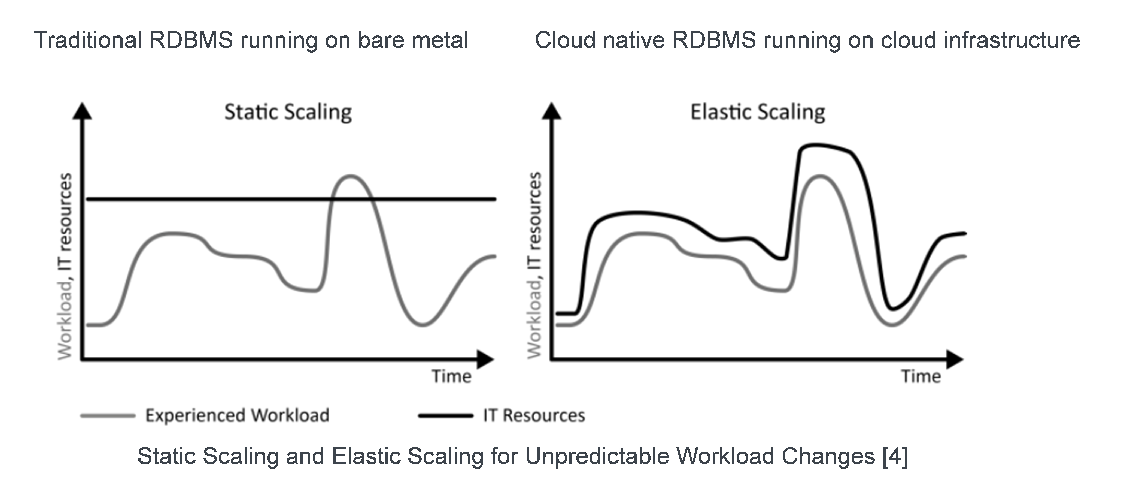
\includegraphics[ width=\linewidth]{figs/elasticScale.eps}
\caption{Elastic scale.} \label{fig8}
\end{figure}

\subsubsection{Kubernetes Stateful Architecture}

\subsubsection{Kubernetes Operator Framework}

\section{Related Work}

\section{Possible Solutions}

\subsubsection{Architecture}

\subsubsection{Design}

\subsubsection{Implementation}

\subsubsection{Test and Evaluation}

\section{Conclusions and Outlook}

\begin{enumerate}
    \item Technology \& Operations
\end{enumerate}
\subsubsection{Acknowledgements} TBD.
%
% ---- Bibliography ----
%
% BibTeX users should specify bibliography style 'splncs04'.
% References will then be sorted and formatted in the correct style.
%
% \bibliographystyle{splncs04}
% \bibliography{mybibliography}
%
\begin{thebibliography}{8}
%%
\bibitem{ref_1} Abraham, R., Brocke, J. v., \& Schneider, J. (2019, July). Data Governance: A conceptual framework, structured review, and research agenda. International Journal of Information Management, 49. \doi{10.1016/j.ijinfomgt.2019.07.008}
%%
\end{thebibliography}
\end{document}